\subsection{Events}
In order to better understand the system, it is necessary to identify the events that may occur, how the system will respond to the event, what caused the event and what type of event it is. For the remote system, the events that may occur are presented in table \ref{table:data}.

\begin{table}[ht]
	\centering
	\resizebox{\columnwidth}{!}{
	\begin{tabular}{||c | c | c | c||} 
		\hline
		\textbf{Event} & \textbf{System Response} & \textbf{Source} & \textbf{Type}\\
		\hline\hline
Login & Show application main screen if successful & Operator & Asynchronous\\\hline
Obtain geolocation & Request device geolocation & Mobile device & Asynchronous\\\hline
App notification & Notifies the operator about the lamppost status & Remote Server & Asynchronous\\\hline
Register operator & Add operator information to databas & Operator & Asynchronous\\\hline
Modify lamppost & Update lamppost information to database & Operator & Asynchronous\\\hline
Register lamppost & Add lamppost information to database & Operator & Asynchronous\\\hline
Insert location	& Show parking spots & User & Asynchronous\\\hline
Obtain geolocation & Request device geolocation & Mobile Device & Asynchronous
		\\\hline
	\end{tabular}
	}
		
	\caption{Remote system events.}
	\label{table:data}
\end{table}


\subsection{Use Cases}
\textbf{Mobile Application}

The mobile application use cases diagram is represented in figure \ref{fig:UseCases_application}, showing that the main actors in the system are the operator, the database and the mobile device. The operator can perform operations such as login, logout, register, modify data about a lamppost and register newly installed posts that are installed, using, for this, the database (to obtain and record data) and the mobile device (to obtain the device location when registering a new post).

\begin{figure}[H]
        \centering
        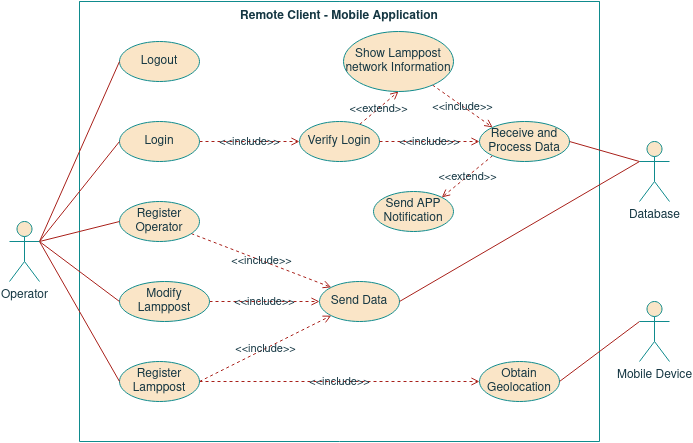
\includegraphics[width=0.85\textwidth]{06remote_system/AppSystem_UseCases}
        \caption{Remote System – Mobile Application Use Cases.}
        \label{fig:UseCases_application}
\end{figure}

\textbf{Web Site}

The web site use cases diagram is shown in figure \ref{fig:UseCases_WebSite}. The main actors are a user, the database and a mobile device. In order to know if there are free parking spaces in a certain location, the user can enter a location (through the street name, for example) or, as in the application, use his mobile device to obtain the location automatically. The database lets the user know where there are empty parking spaces.

\begin{figure}[H]
        \centering
        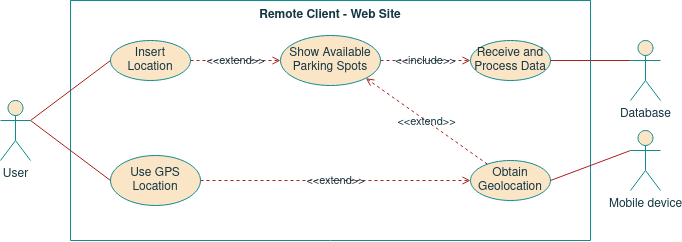
\includegraphics[width=0.75\textwidth]{06remote_system/WebSite_UseCases}
        \caption{Remote System – Web Site Use Cases.}
        \label{fig:UseCases_WebSite}
\end{figure}

\subsection{State Chart}
\textbf{Mobile Application}

In the figure \ref{fig:StateChart_application} is represented the state chart of the mobile application. It initiates with the system configuration, showing a home screen that allows the operator, the application user, to log into the system or register himself, if he doesn’t have login credentials. After a successful login, the system will show information about the lampposts associated to the logged in operator and he can do operations like register lampposts, modify lampposts information and logout of the system.

\begin{figure}[H]
        \centering
        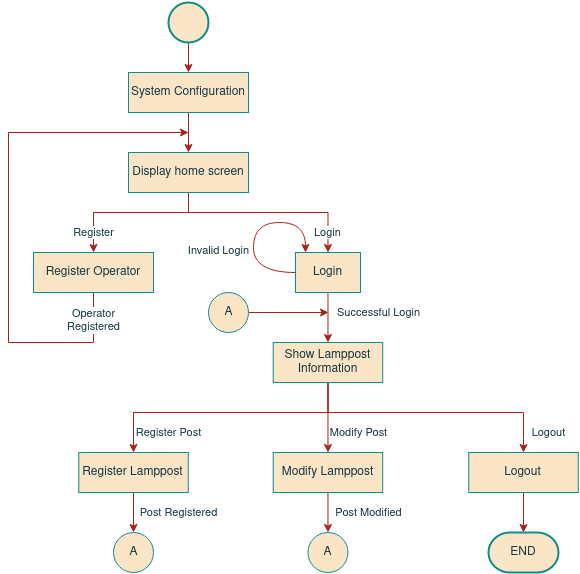
\includegraphics[width=1\textwidth]{06remote_system/AppSystem_StateChart}
        \caption{Remote System – Mobile Application State Chart.}
        \label{fig:StateChart_application}
\end{figure}

\textbf{Web Site}

In figure \ref{fig:StateChart_WebSite}, one can see the web site state chart. The system initiates with the system configuration. Then it asks the user if he wants to use his location (through the mobile phone's GPS tracking system) or type manually the location. If the user enters the location manually (the street name, for example), it will be checked and, if valid, the free parking spaces will be displayed.

\begin{figure}[H]
        \centering
        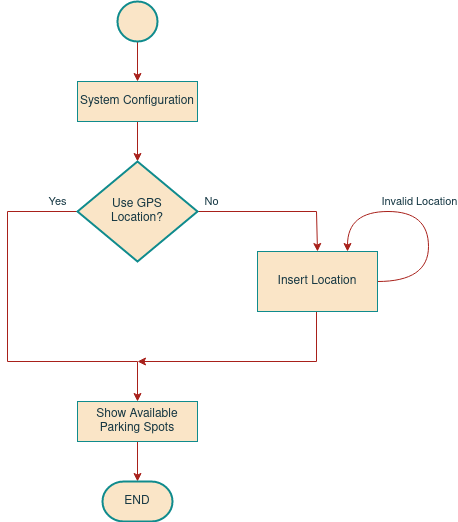
\includegraphics[width=0.75\textwidth]{06remote_system/WebSite_StateChart}
        \caption{Remote System – Web Site State Chart.}
        \label{fig:StateChart_WebSite}
\end{figure}

\subsection{Sequence Diagram}
\textbf{Mobile Application}

In figure \ref{fig:SeqDiagram_application}, one can see the web site state chart. The system initiates with the system configuration. Then it asks the user if he wants to use his location (through the mobile phone's GPS tracking system) or type manually the location. If the user enters the location manually (the street name, for example), it will be checked and, if valid, the free parking spaces will be displayed.

\begin{figure}[H]
        \centering
        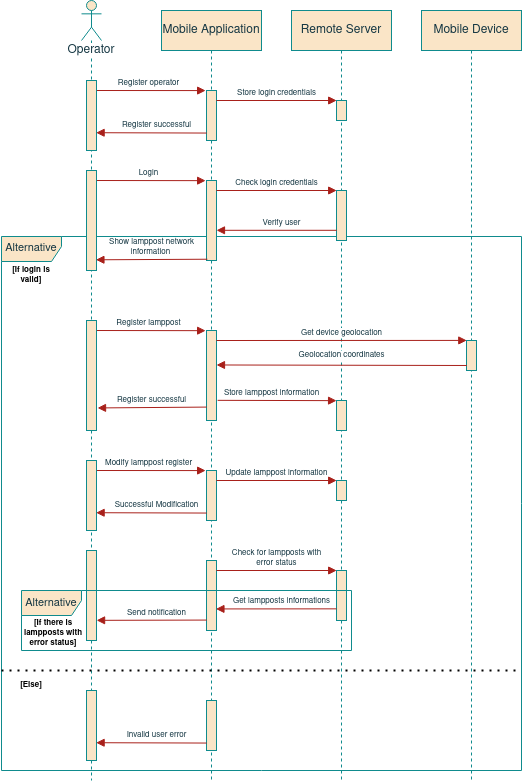
\includegraphics[width=0.75\textwidth]{06remote_system/AppSystem_SeqDiagram}
        \caption{Remote System – Mobile Application Sequence Diagram.}
        \label{fig:SeqDiagram_application}
\end{figure}

\textbf{Web Site}

The sequence diagram of the web site is shown in the figure \ref{fig:SeqDiagram_WebSite}. To know where there are empty parking spots, the user can insert manually a location or use his \ac{gps} location. In both cases the web site asks the remote server (database) if there are available parking spots near the location and displays them to the user. However, in the case of using the \ac{gps} location, the web site has to get the \ac{gps} coordinates from the mobile device running the web site.

\begin{figure}[H]
        \centering
        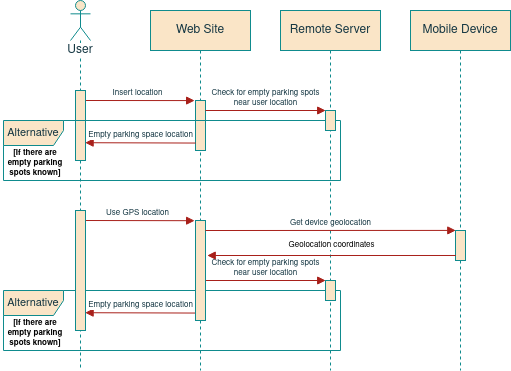
\includegraphics[width=0.75\textwidth]{06remote_system/WebSite_SeqDiagram}
        \caption{Remote System – Web Site Sequence Diagram.}
        \label{fig:SeqDiagram_WebSite}
\end{figure}